\section{System's Perspective}
%The report doesn't need to be structured in subsections to answer each question. The most important is that all these questions are answered in some way throughout the System's perspective section.
In the sections below, the architecture and deployment specifications of the MiniTwit system will be covered.

\subsection{Architecture and Design}

\subsubsection{Overview}
Below is the deployment diagram of the complete system hosted with Docker on DigitalOcean:

\begin{figure}[h!]
    \centering
    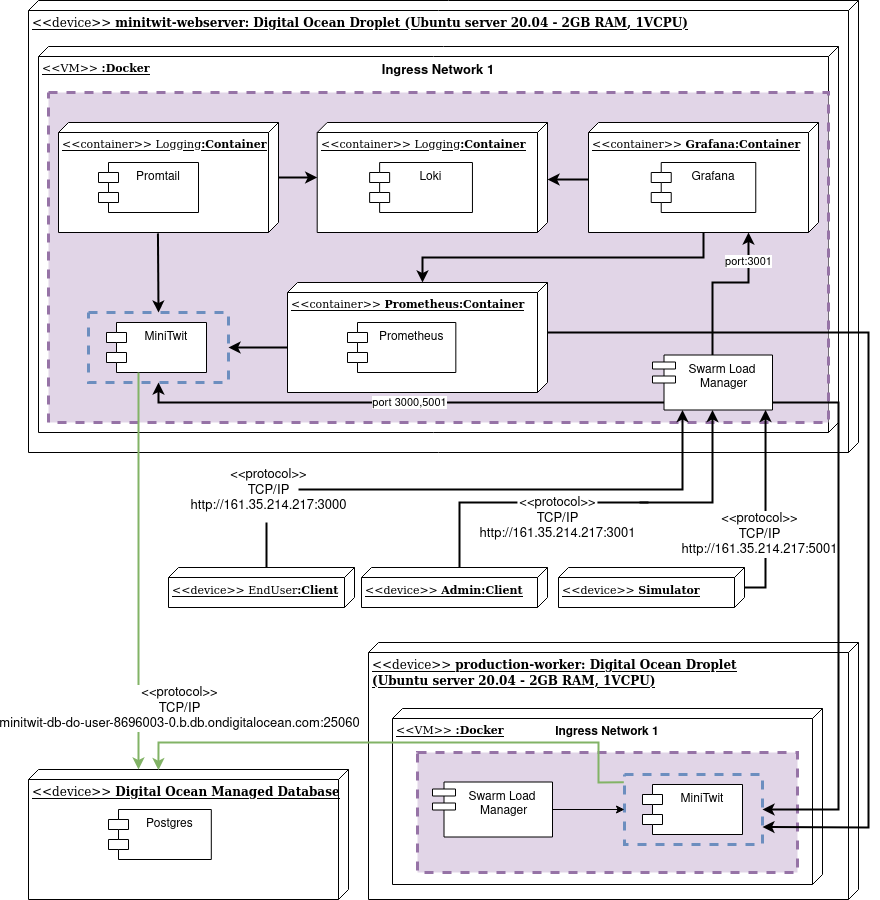
\includegraphics[width=1\linewidth]{report/images/system-architecture.png}
    \caption{System Architecture \href{https://github.com/Niels-Frederik/MiniTwit/blob/main/report/images/system-architecture.png}{(Click to see full size image)}}
    \label{fig:arcitechture-overview}
\end{figure}

\noindent Green arrow: database connection. \\
Blue dashed rectangle: containers abstracted into a component for readability.

\noindent
The MiniTwit application runs on two droplets on Digital Ocean. A managed database, hosted on Digital Ocean, is hosting a Postgres database. The \textit{minitwit-webserver} droplet is running in Docker swarm mode, and functions as a swarm manager \cite{docker-swarm}. The \textit{production-worker} droplet is a worker node within this swarm. The swarm hosts the MiniTwit component in four replicas. Furthermore, the swarm hosts the monitoring and logging stack in a single replica. This stack consists of Promtail and Loki to fetch and aggregate logs, Prometheus to collect and perform metric querying, and finally Grafana to display the monitored and logged data. The swarm is run with a docker-compose.yml file, which can be seen in appendix \ref{appendix:docker-compose}. \\
Lastly, the swarm utilizes DockerHub to pull all images for the different services.\\
\\
The MiniTwit component depicted, is an abstraction to increase readability in the UML drawing. It is therefore not a single container hosted in the swarm, but rather a component consisting of multiple services. Herein located; front-end, Sim-API for the simulator, and the API for the front-end.
Figure \ref{fig:minitwit-decomposition} below is a decomposition of this MiniTwit component:

\begin{figure}[H]
    \centering
    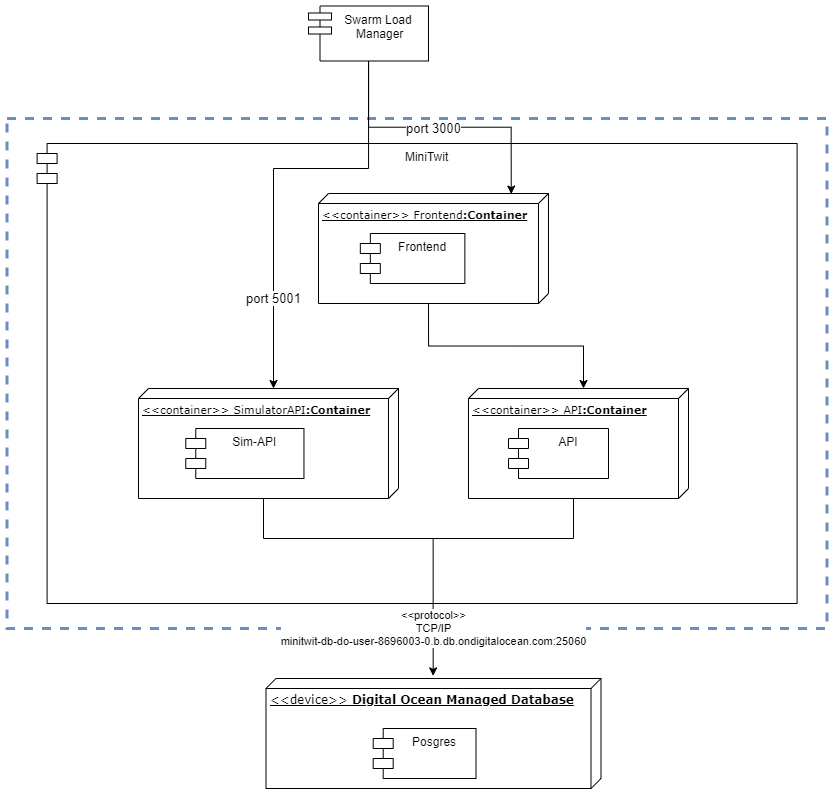
\includegraphics[width=1\linewidth]{report/images/minitwit-decomposition.png}
    \caption{MiniTwit Component Decomposition}
    \label{fig:minitwit-decomposition}
\end{figure}

\subsubsection{Design Choices}

%TA used 3+1 view model. 
%Deployment diagram should be enough. 
%Maybe add package diagram - of how the API works with the different components.

The \textit{Frontend} service is written in React.js. Both the \textit{Sim-API} and \textit{API} runs on \textit{Node.js} and exposes a RESTful API implemented with \textit{Express.js}. \\
The rationale behind using JavaScript was mainly due to its lightweight approach compared to e.g. C\#. Furthermore, the team wanted to have experience with a new language and frameworks. Lastly, developing with JavaScript is quick and eases the development process through libraries like Nodemon, which allows for recompilation at run-time.
The component diagram of the back-end can be seen below in figure \ref{fig:back-end-component-diagram}:

\begin{figure}[H]
    \centering
    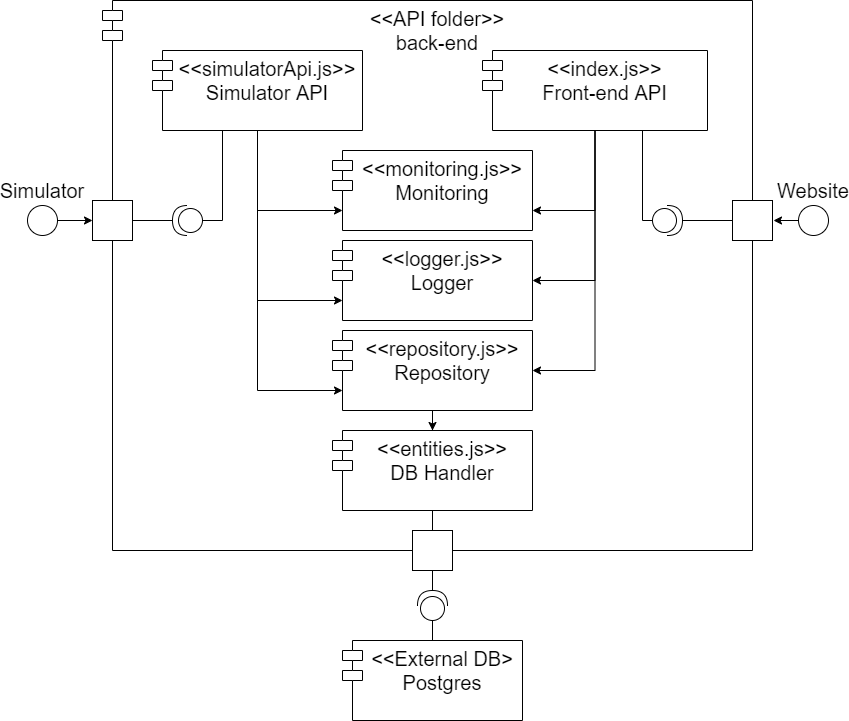
\includegraphics[width=1\linewidth]{report/images/component-diagram.png}
    \caption{Back-end Component diagram}
    \label{fig:back-end-component-diagram}
\end{figure}

\noindent
Each component in the back-end is represented by a single file. Both APIs implement the same endpoints, and uses the rest of the components as helpers to resolve each request.\\
The following list briefly describes each component:
\begin{enumerate}
    \item \textbf{Monitoring:} Provides functionality to collect metrics used by Prometheus
    \item \textbf{Logger:} Provides logger objects to perform logging by utilizing the \textit{winston} and \textit{express-winston} libraries.
    \item \textbf{Repository:} Provides a repository object, which uses Sequelize to query the database.
    \item \textbf{DB Handler:} Provides a Sequelize ORM object to query the database.
\end{enumerate}

A Postgres database was chosen due to the team's previous experience, and because of its relational nature, which fits the purpose of this project. The Sequelize library is used in the \textit{DB Handler} as the database abstraction layer. It was chosen because it is well documented \cite{sequelize}, and has a large community on Stackoverflow.

\newpage
\subsection{Dependencies}
This section will cover all the dependencies in the system on all layers of abstraction.

\subsubsection{Front-end and Back-end Low Level Diagrams}
The following is a description of the syntax used in the next two diagrams:
\begin{itemize}
    \item Squares: files developed by the team
    \item Circles: external libraries
    \item Arrow: build-/compile-time dependency
    \item Dashed arrow: run-time dependency
\end{itemize}

\noindent The Front-end has the following Dependencies:
\begin{figure}[H]
    \centering
    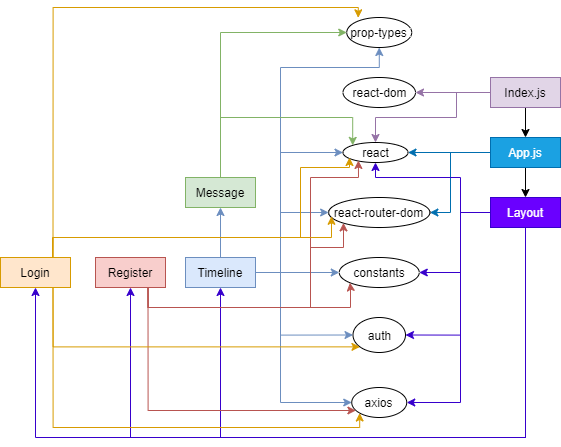
\includegraphics[width=0.9\linewidth]{report/images/Frontend-dependencies.png}
    \caption{Front-end dependency diagram}
    \label{fig:front-end-depencency-diagram}
\end{figure}
The squares represent React components. Colors are used to improve readability. \\
The source code represented in this diagram is located in the Minitwit/Frontend folder. The exact versions of all frontend dependencies can be seen in appendix \ref{appendix:front-end-dependencies}

\newpage
The back-end has the following dependencies:
\begin{figure}[H]
    \centering
    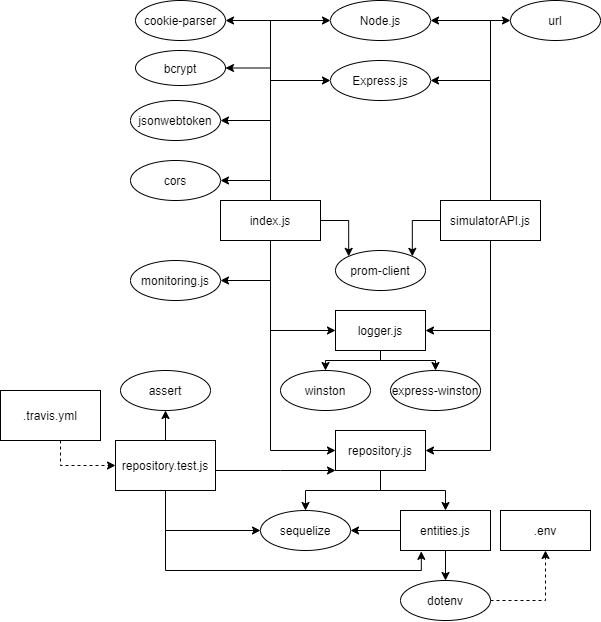
\includegraphics[width=1\linewidth]{report/images/backend-dependencies.png}
    \caption{Back-end dependency diagram}
    \label{fig:back-end-depencency-diagram}
\end{figure}

\noindent
The source code represented in this diagram is located in the Minitwit/API folder. The API used when accessing the system through the webpage is handled by the \textit{index.js} file, while the simulator uses the \textit{simulatorAPI.js} file.\\
All dependencies in the front-end and back-end use the latest major release, e.g. the \textit{bcrypt} dependency uses \^{}5.0.0, meaning all releases up until the next major release: v6.0.0. \\
The exact versions of all backend dependencies can be seen in appendix \ref{appendix:back-end-dependencies}

\subsubsection{The Whole System}
The following describes the syntax used in the diagram:
\begin{itemize}
    \item Full line arrow: dependency
    \item Stippled line arrow: retired dependency
    \item Colored line arrow: for readability purpose only
\end{itemize}

\begin{figure}[H]
    \centering
    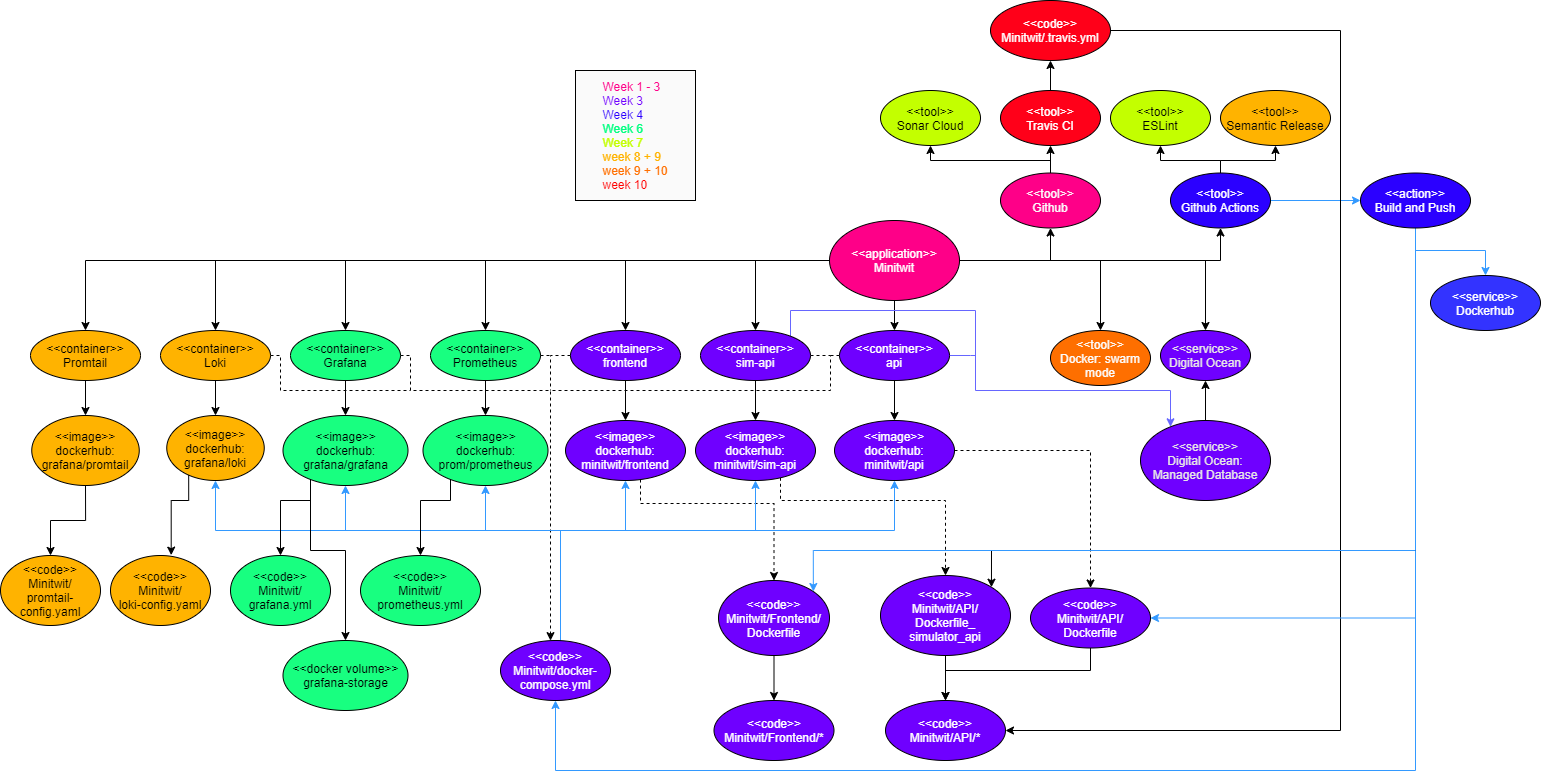
\includegraphics[scale=0.25]{report/images/system-dependencies.png}
    \caption{System dependencies. \href{https://github.com/Niels-Frederik/MiniTwit/blob/main/report/images/system-dependencies.png}{Click here for full size image}}
    \label{fig:system-depencencies}
\end{figure}

The diagram displays the dependencies of the project at a high level of abstraction. The various dependencies are color-coded, such that the color corresponds to the week, the dependency was introduced. 
\\
The dependencies of the front-end and back-end are omitted as they are described in figure \ref{fig:front-end-depencency-diagram} and \ref{fig:back-end-depencency-diagram}.

\subsection{The Current State of The System}
SonarCloud provides an overview of the general code quality for the MiniTwit application as seen in figure \ref{fig:sonarcloud} below:

\begin{figure}[H]
    \centering
    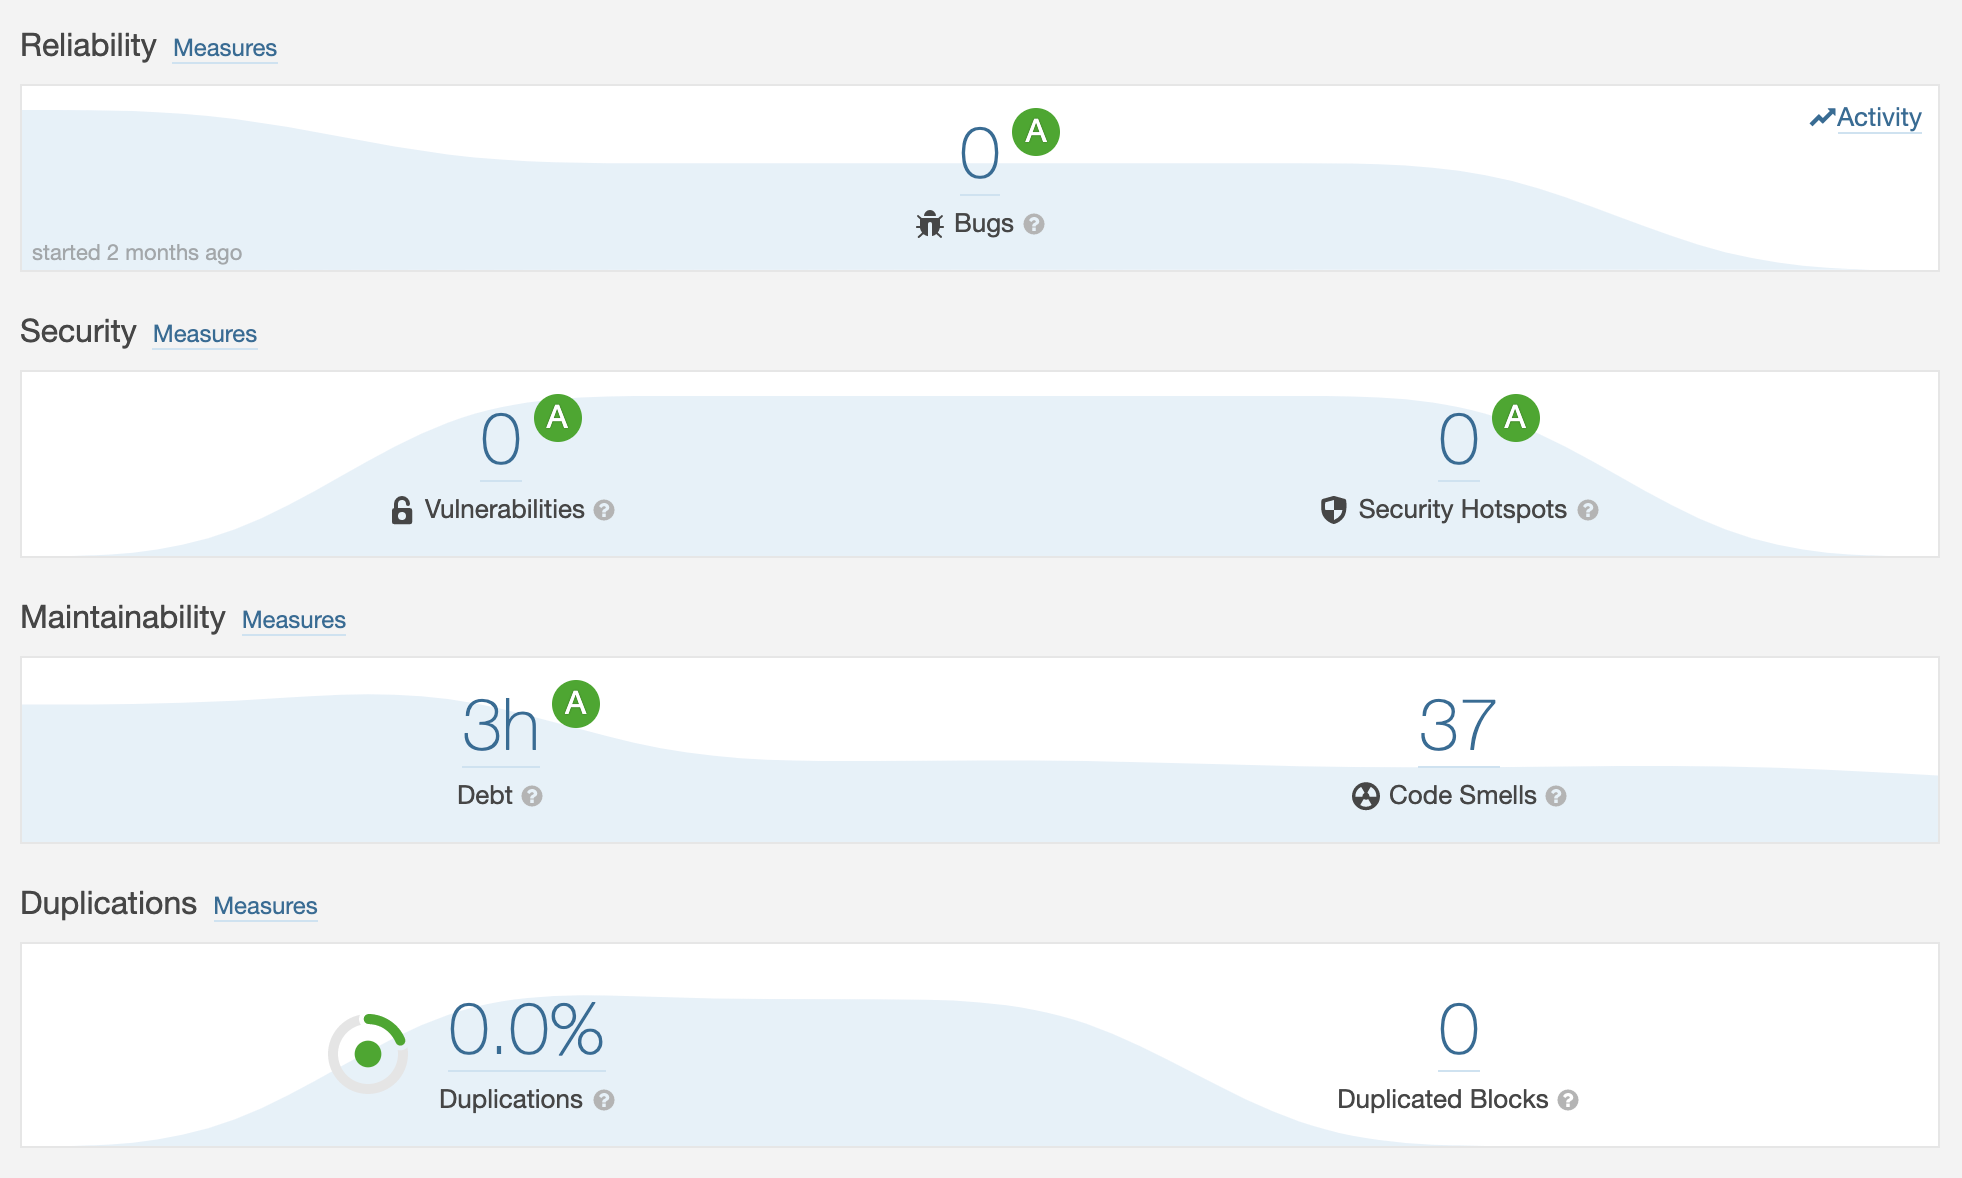
\includegraphics[width=0.90\linewidth]{report/images/SonarCloudOverview.png}
    \caption{SonarCloud overview of code quality}
    \label{fig:sonarcloud}
\end{figure}

\noindent
From this overview, it is seen that the state of the system is as desired, with room for improvement on the maintainability measures. For this project, SonarCloud shows an estimated technical debt of 3 hours distributed between 37 code smells. The code smells mainly comprise of outcommented code, which is solved simply by removing it. SonarCloud estimates the time consumption to solve each of these code smells to be 5 minutes, which makes the technical debt seem higher than what it is in reality:

\begin{figure}[H]
    \centering
    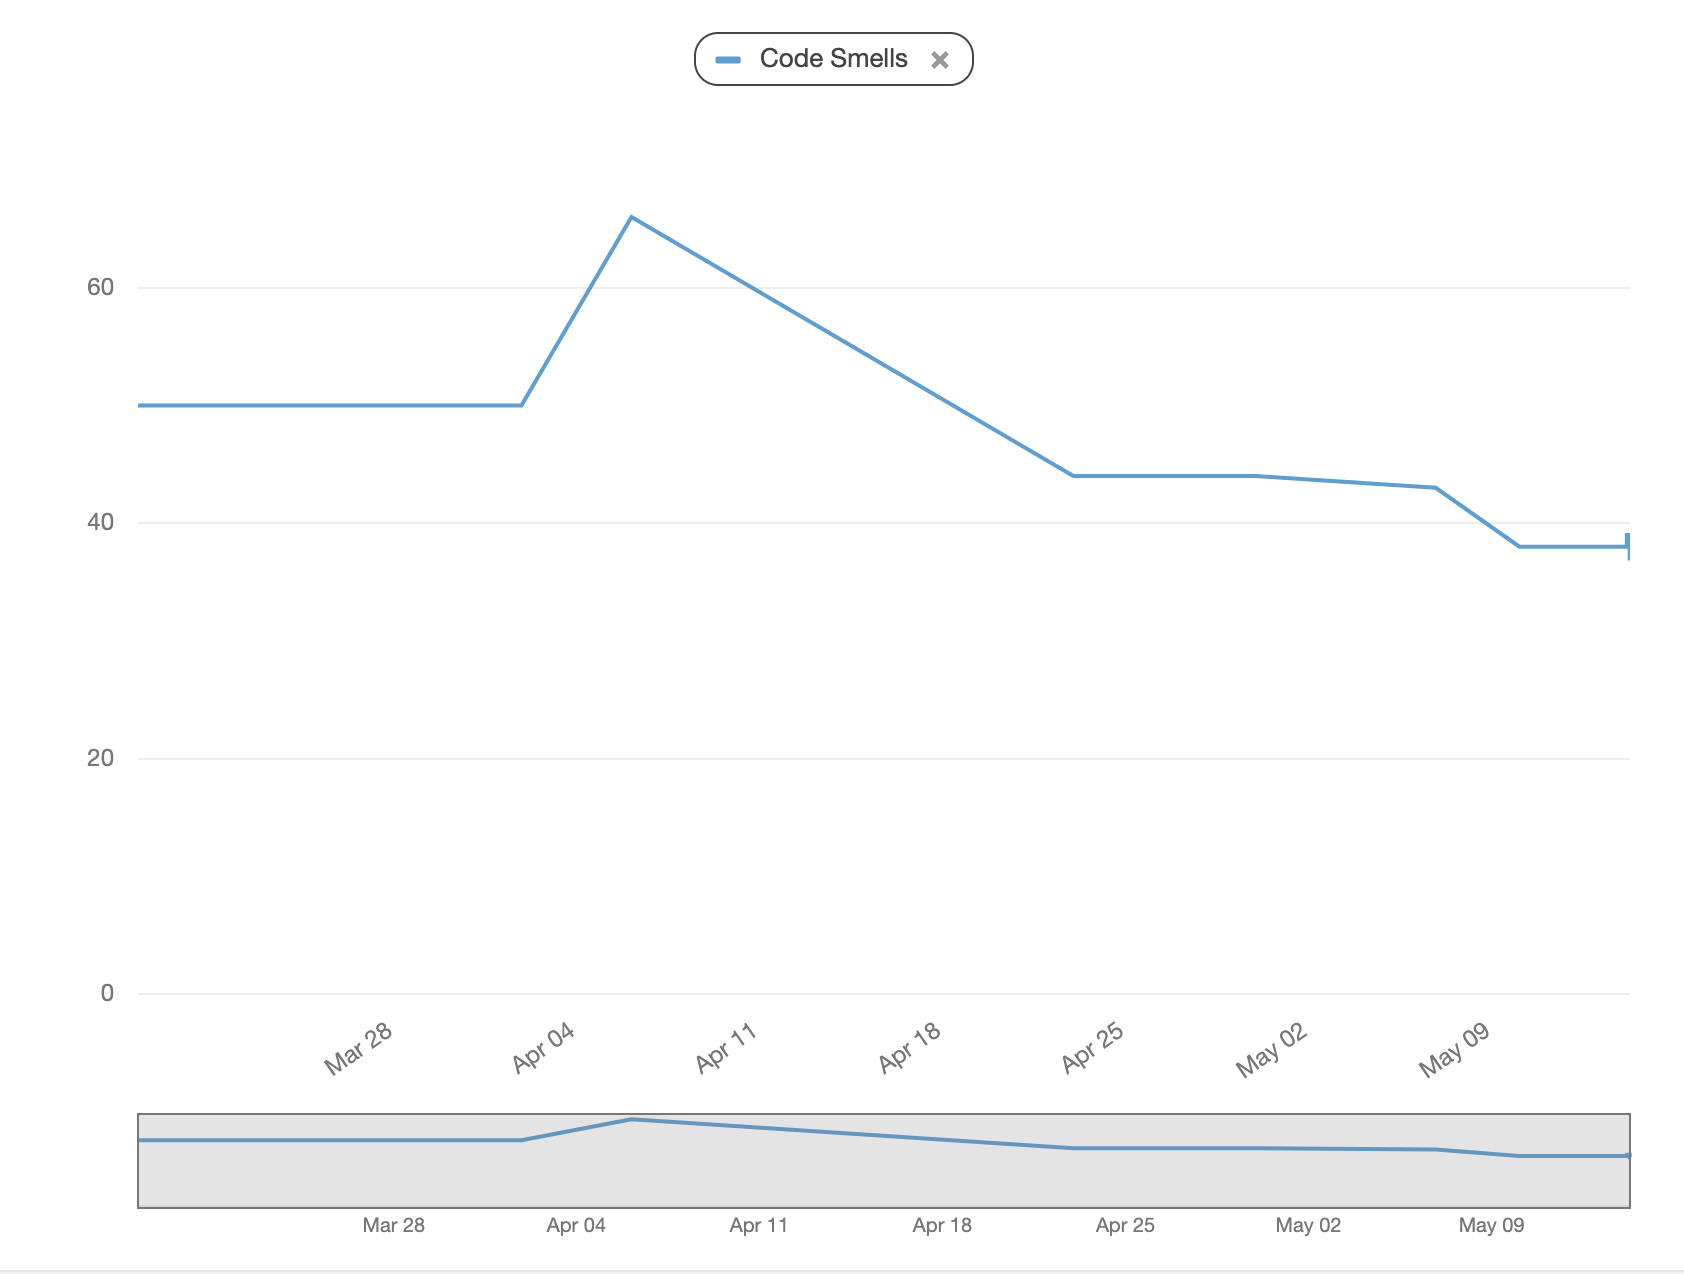
\includegraphics[width=0.90\linewidth, height=0.6\linewidth]{report/images/SonarCloudCodeSmells.png}
    \caption{Amount of code smells per date}
    \label{fig:sonarcloudsmells}
\end{figure}

\noindent
As seen in figure \ref{fig:sonarcloudsmells}, the number of code smells has steadily decreased since adding ESLint to the pipeline, which will be elaborated in section \ref{CI/CD}. To secure less code smell in the future, ESLint could have been configured to be more strict. 



\subsection{License}
The ScanCode toolkit\cite{scancode} was used to scan for all licenses within the MiniTwit repository. The scan here outputted several permissive licenses, where the most relevant were MIT and Apache-2.0. Furthermore, the most important finding was that no version of the GPL license was present. This is important, as the GPL is a copyleft license that would require MiniTwit to be a free open-source license\cite{gpl}. Hence, since no copyleft licenses such as GPL are in the project, MiniTwit has a variety of licenses to choose from.\\
The group chose the permissive MIT license to provide everyone with the free right to use the API, as well as keeping the developer team free from being liable for any claims made against any possible damage caused by the API.

\subsection{Service Level Agreement}
The SLA can be found  \href{https://github.com/Niels-Frederik/MiniTwit/blob/main/API/SLA.md}{\underline{here}}.
\\
The SLA mentions that the API guarantees an up-time of 99.99\%. This metric is calculated by the following equation:

\[
    UpTimePercentage = \frac{Total Transaction Attempts - Failed Transactions}{Total Transaction Attempts}
\]
Due to an error causing stored monitored data to be wiped prior to the the 14th. of May, the following data from 14/05 - 17/05 was used for the calculation:\\
\begin{figure}[H]
    \centering
    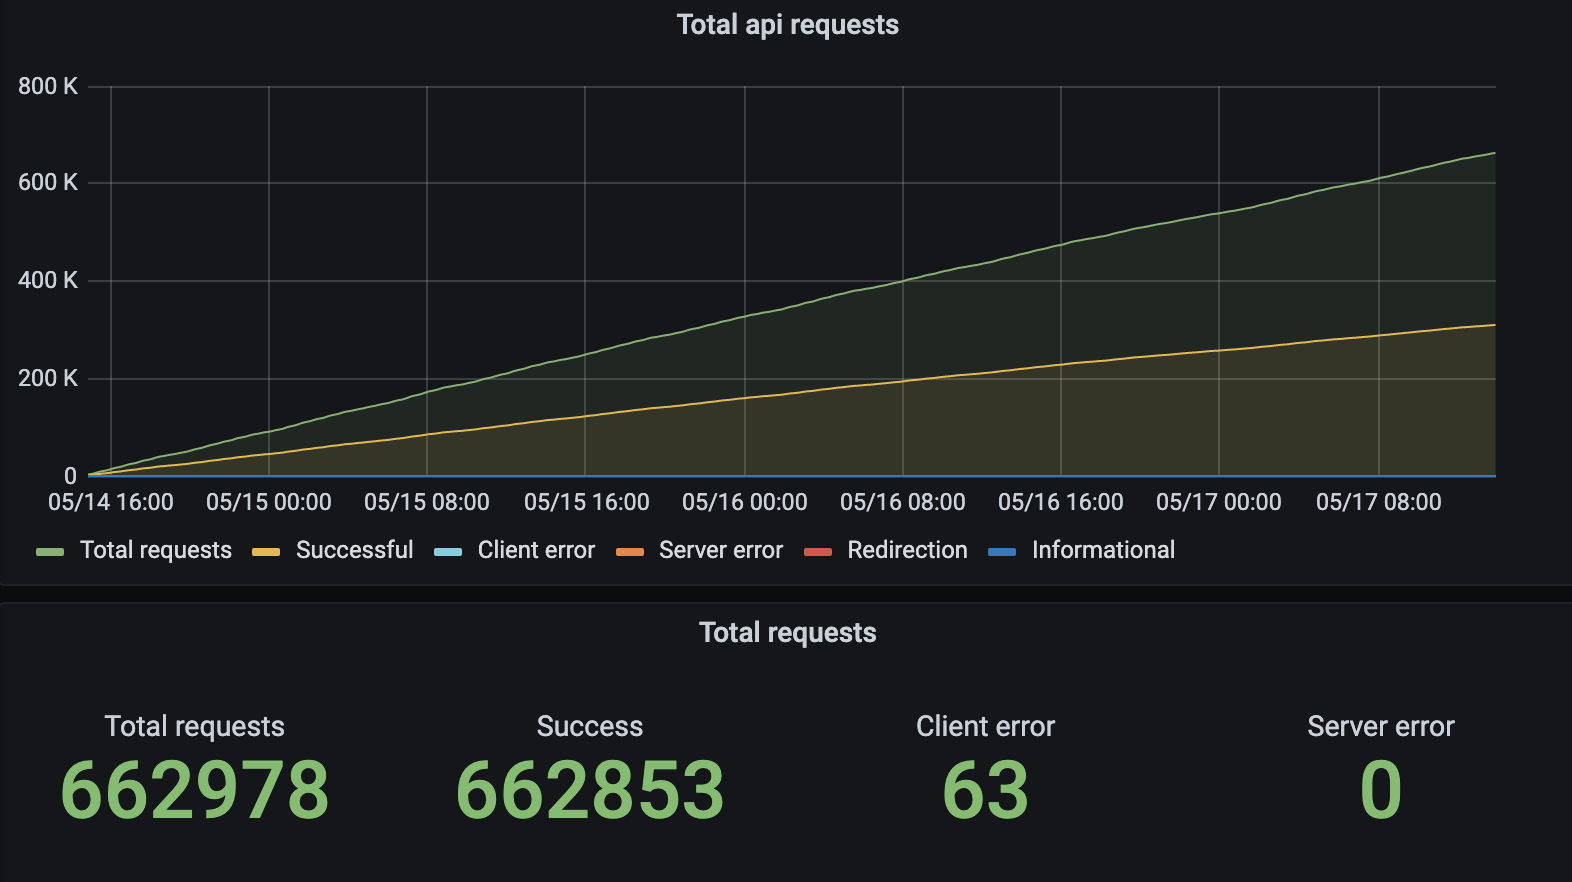
\includegraphics[width=0.90\linewidth]{report/images/sla_metrics.png}
    \caption{Total requests 14/05 - 17/05}
    \label{fig:totalrequests}
\end{figure}

\noindent
We here chose to count all of the client errors as Failed Transactions as the client errors were caused by users not being registered in the MiniTwit application due to a server error. Hence, the 99.99\% is derived from the following:
\[
    99.99\% = \frac{(662978 - 63)}{662978}
\]

\noindent
Furthermore, the SLA states a response time on POST and GET messages. It here states a POST response time varying from $\sim$0.0250s to $\sim$1.02s and a maximum GET response time of 100ms. Both of these are derived from the following figure: \ref{fig:Monitoring2}